\documentclass[11pt,a4paper]{article}
\usepackage[utf8]{inputenc}
\usepackage[spanish]{babel}	%Idioma
\usepackage{amsmath}
\usepackage{amsfonts}
\usepackage{amssymb}
\usepackage{graphicx} %Añadir imágenes
\usepackage{geometry}	%Ajustar márgenes
\usepackage[export]{adjustbox}[2011/08/13]
\usepackage{float}
\restylefloat{table}
\usepackage{hyperref}
\usepackage{titling}
\usepackage{minted}
\usepackage{multicol}
%Opciones de encabezado y pie de página:
\usepackage{fancyhdr}
\pagestyle{fancy}
\lhead{}
%\rhead{}
\lfoot{Técnicas de los Sistemas Inteligentes}
\cfoot{}
\rfoot{\thepage}
\renewcommand{\headrulewidth}{0.4pt}
\renewcommand{\footrulewidth}{0.4pt}
%Opciones de fuente:
\renewcommand{\familydefault}{\sfdefault}
\setlength{\parindent}{0pt}
\setlength{\headheight}{12pt}
\setlength{\voffset}{10mm}

% Custom colors
\usepackage{color}
\definecolor{deepblue}{rgb}{0,0,0.5}
\definecolor{deepred}{rgb}{0.6,0,0}
\definecolor{deepgreen}{rgb}{0,0.5,0}

\usepackage{listings}

\pretitle{%
  \centering
  \LARGE
  
\includegraphics[scale=0.5]{img/logo.png}\\[\bigskipamount]
}
\posttitle{\begin{center} \end{center}}

\author{	Juan Ocaña Valenzuela}
\title{\textbf{Práctica 2: planificación clásica en PDDL}}

\begin{document}

\thispagestyle{empty}

\maketitle

\newpage

\tableofcontents

\newpage

\section{Diario de trabajo}

\subsection*{Domingo, 5 de mayo de 2019}
Empecé la práctica hace unos días, pero no ha sido hasta hoy que he decidido comenzar a documentarla.
Llevaba unos días bastante ocupado (la fiesta de la Escuela no se organiza sola), y tenía visita en casa, así que dedicaba
relativamente poco espacio de mi sistema nervioso central a pensar en los apasionantes mundos de Belkan, más allá de la 
eterna duda: ¿es Belkan el personaje? ¿es el nombre del mundo? ¿o quizá un ser omnipresente que gobierna por aquellos lares?


Una vez mi visita se marchó, comencé a plantear el primer ejercicio de la relación, diseñando un mapa, poniendo cosas en él,
definiendo las acciones y todo eso. Una vez creí haber terminado el modesto problema 1, en el cual cada personaje debe tener un
objeto, ejecuté FF y...


\textbf{no funcionaba.}

\bigskip

No encontraba un plan. No lo encontraba y no sabía por qué. Estaba cansado y no me apetecía hacer nada, así que mandé a la
mierda los estrafalarios mundos de Belkan y me puse a jugar a Persona 5.

\medskip

Hoy es un día nuevo, y nada más levantarme y desayunar he pensado que quizás podría hacer un pequeño esfuerzo por saber 
qué le pasaba a mi problema, y cómo arreglarlo. Y es que nuestro pequeño bicho no puede entregar objetos a los personajes
si no lo hemos definido en el problema. Qué cosas, eh.

\medskip

Bautizado como Patrick Dotimas (Patrick para los amigos), ahora que está en el problema encuentra una solución.
Ya tenemos un problema resuelto... O no.

\medskip

Observando el plan, resulta que, en un acto de amor incondicional, Patrick se entrega a sí mismo a los personajes, y no los
objetos que coge. En lugar de algo como:

\medskip
\begin{center}
\texttt{GIVE PATRICK ROSE R20 PRINCESS}
\end{center}

\medskip

tenemos algo así:

\medskip
\begin{center}
\texttt{GIVE PATRICK PATRICK R20 PRINCESS}
\end{center}

\medskip

A ver cómo lo soluciono... De momento voy a comer.

\bigskip

\textbf{[Actualización - 19:30]}

Después de procrastinar un buen rato (y jugar otro rato a Persona 5), me he dado cuenta de que el dominio no
estaba mal del todo. Patrick cogía sus objetos y los entregaba bien, pero no sabía qué objeto tenía ni daba.
Lo he solucionado añadiendo un predicado más, \texttt{on\_hand}, que viene explicado en su sitio.

\medskip

Acabo de caer en una cosa... Si Belkan es el personaje, y nuestro jugador se llama Patrick, 
¿son estos los extraños mundos de Patrick? 
En fin, voy a ponerme con el generador de problemas, a ver si marcha. 

\medskip

\subsection*{Sábado, 11 de mayo de 2019}
Tras la fiesta de la escuela uno se encuentra destrozado y libre a partes iguales, así que seguir con la práctica
era una buena idea. Me puse con el parser de los dos primeros ejercicios, y tras darle algunas vueltas me creaba problemas 
que deberían funcionar pero no lo hacían. ¿Por qué? Por los paréntesis. Siempre son los paréntesis.

\subsection*{Miércoles, 15 de mayo de 2019}
Los ejercicios tres y cuatro han sido fáciles, pero el parser del ejercicio cuatro me parece poco claro. 
Según el enunciado hay que leer el número de puntos a conseguir, pero introducir la tabla de puntos en el problema no es tan
trivial como parecía al prinicipio. En fin, es lo que hay.

\subsection*{Domingo, 19 de mayo de 2019}
Me he dado cuenta de que plantear los ejercicios en PDDL es más sencillo que hacer el parser en la mayoría de las ocasiones.
Los ejercicios cinco y seis han consistido en modificar un par de cosas de los dominios anteriores, mientras que el parser cada
vez se complica más (aunque tampoco demasiado).

\subsection*{Martes, 21 de mayo de 2019}
Doy por terminado el trabajo que voy a entregar. Podría hacer más, pero tengo más cosas que hacer y creo que es suficiente y funciona
moderadamente bien.

\subsection*{Miércoles, 22 de mayo de 2019}
Procedo a documentar la práctica. Hay más trabajo del que parece, ya que hay que poner las cosas bonitas, dibujar un par de mapas, explicar los ejercicios, etc. Pero bueno, es echarle un rato. Lo peor ya ha pasado.

\section{Leyenda}

En los mapas adjuntos se representan los elementos del dominio de la siguiente forma:

\textbf{Objetos:} escritos en gris, sobre la zona en la que se encuentran.
\textbf{Personajes:} escritos en negro, sobre la zona en la que se encuentran.
\textbf{Distancia entre zonas:} representada sobre la unión de las zonas.
\textbf{Tipo de zona:} representada por el color de la zona:
\begin{itemize}
\item \textbf{Azul:} agua.
\item \textbf{Marrón claro:} arena.
\item \textbf{Marrón oscuro:} piedra.
\item \textbf{Gris oscuro:} precipicio.
\item \textbf{Verde:} bosque.
\end{itemize}

\section{Ejercicios}

\subsection{Ejercicio 1}

Definir  un  dominio y  problema de  planificación considerando  que  el  jugador podrá    estar  orientado  al  norte,  sur,  este  u  oeste  y  desplazarse  de  una  zona  a  otra siempre  que  esté  correctamente  orientado.  Por  ejemplo,  podrá  desplazarse  a  una zona  al  norte  de  su  zona  actual,  si  está  orientado  al  norte.

\subsection{Mapa problema 1}
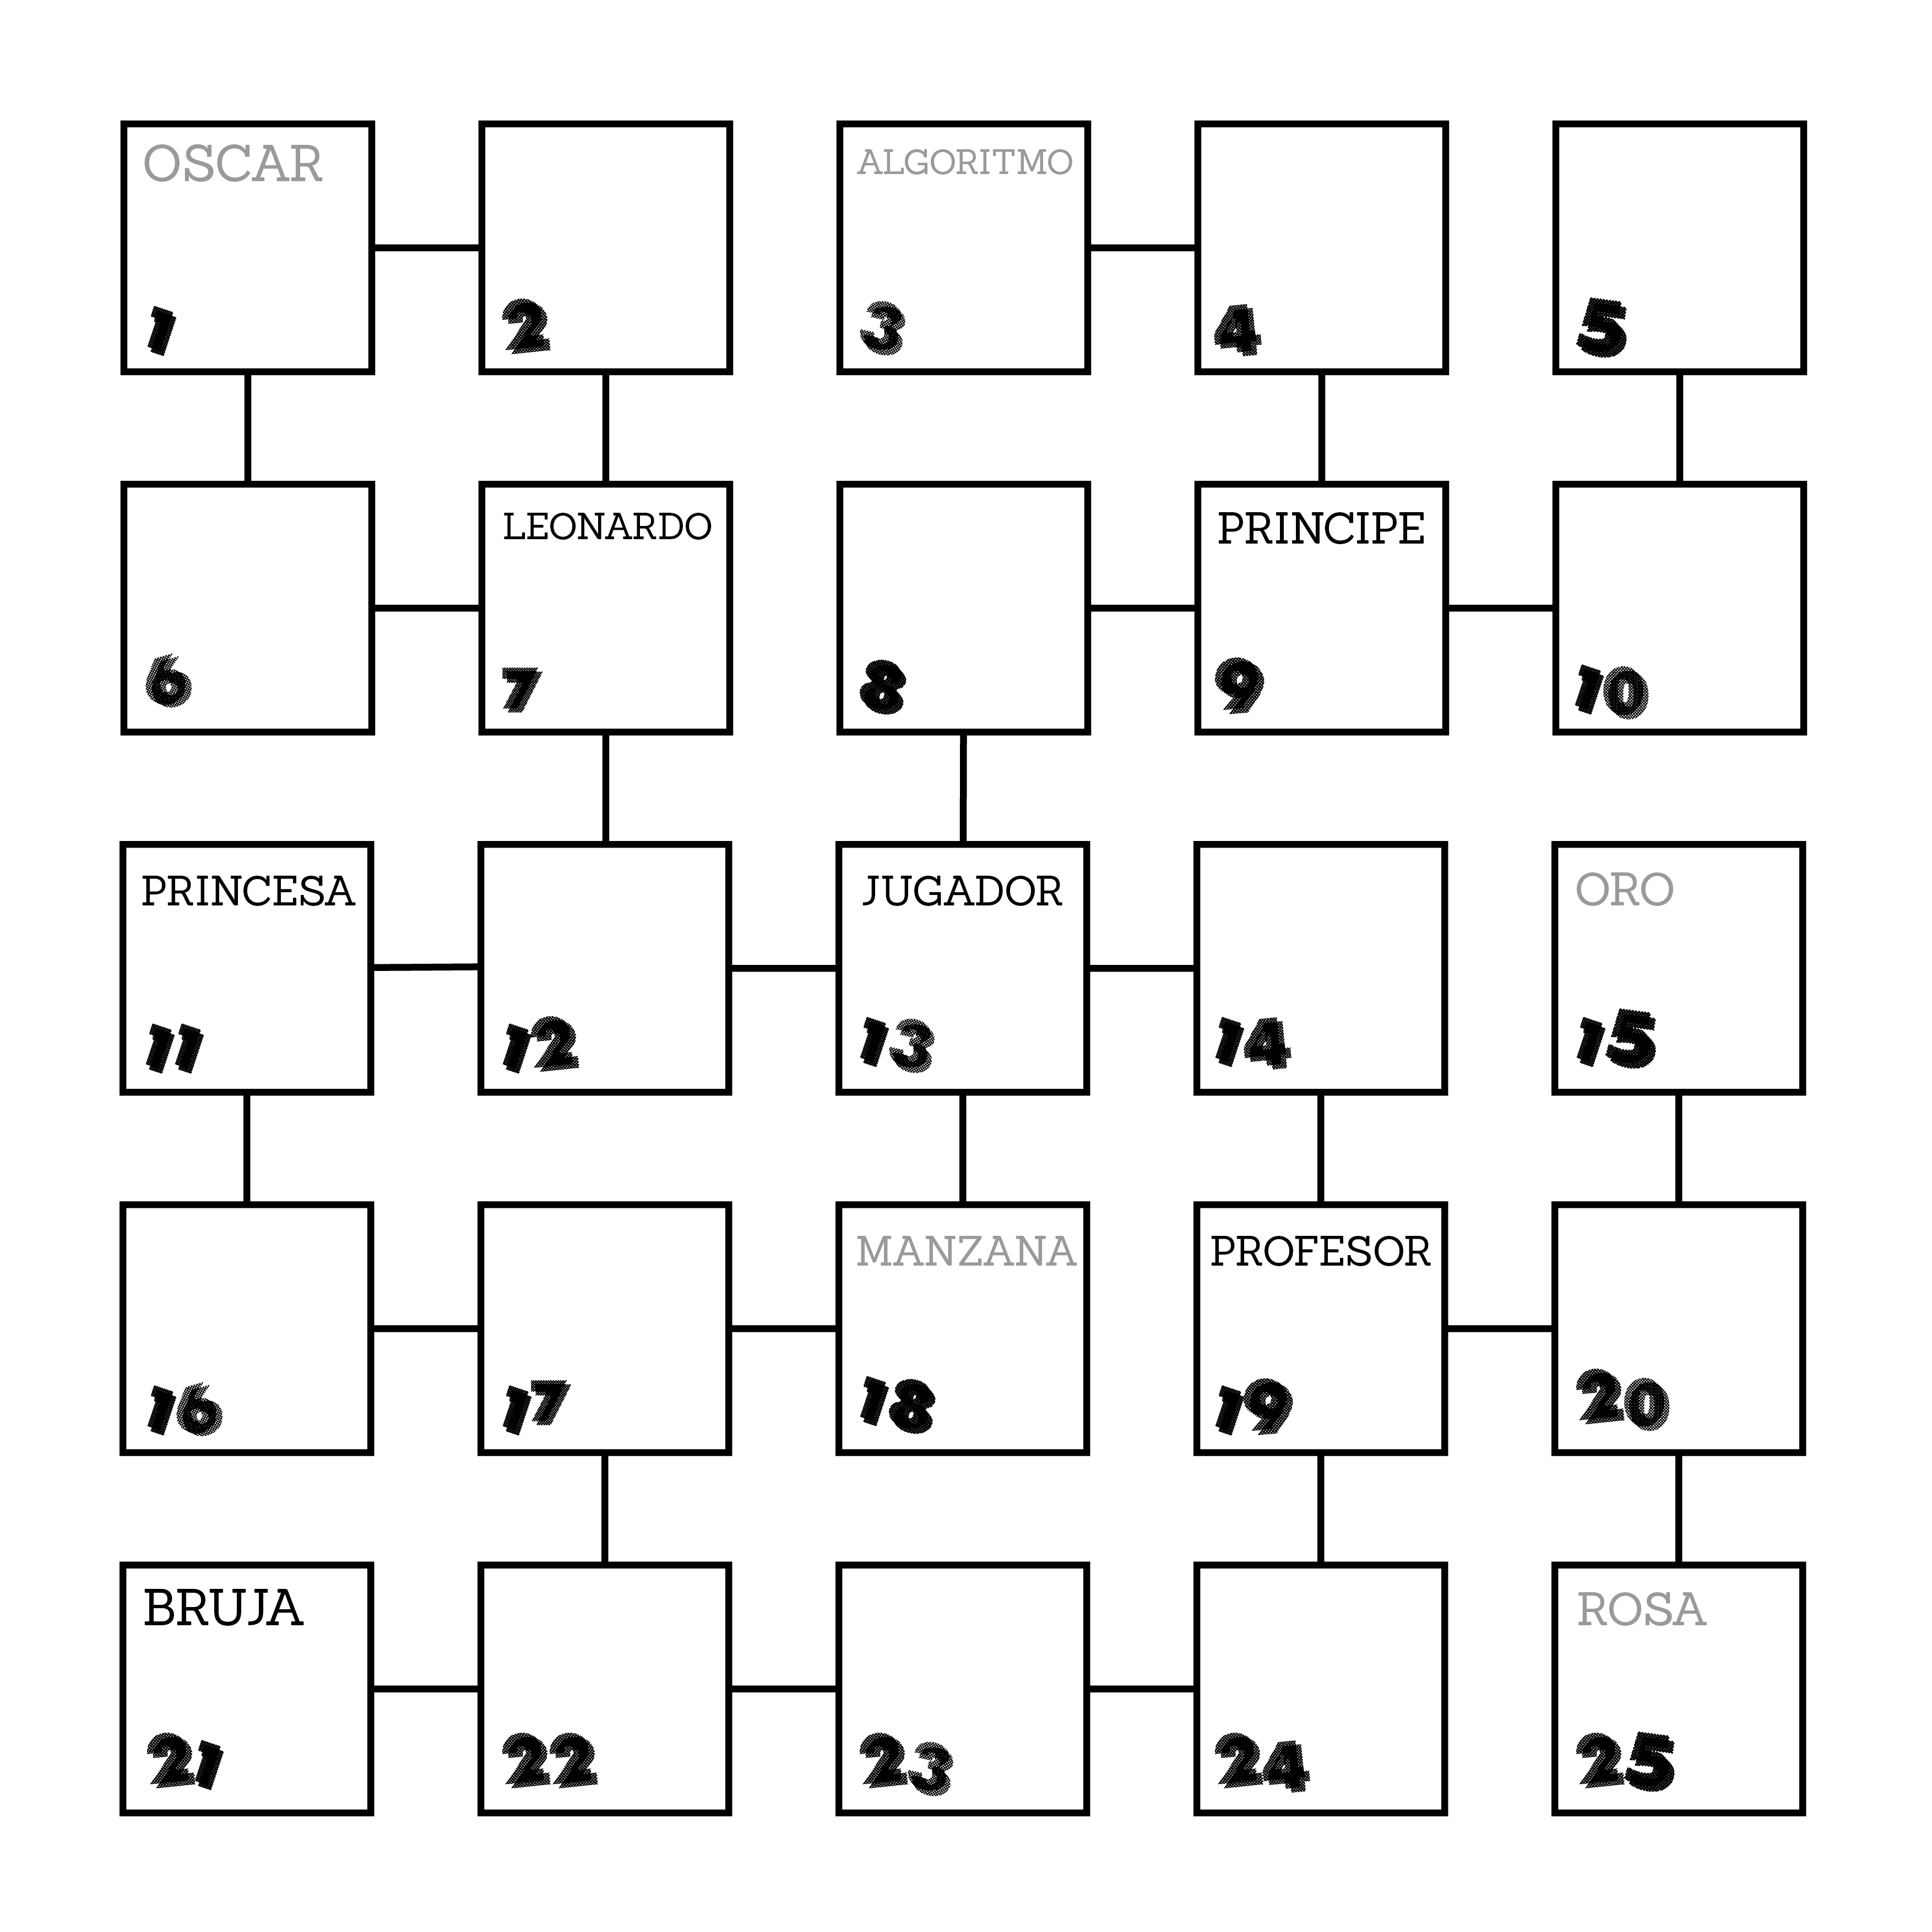
\includegraphics[scale=0.5]{img/e1.png}
\subsubsection{Apartado A}

\textbf{Representar en el dominio los objetos del mundo.}

\bigskip

Para representar los objetos del mundo (jugador, personajes, objetos, habitaciones, caminos, etc.) se han establecido
los siguientes tipos, con su jerarquía:

\medskip

\textbf{locatable:} elemento que se puede localizar en una posición.
	
\quad \textbf{character:} personaje.

\quad \quad	\textbf{player:} jugador.

\quad \quad \textbf{npc:} personaje no jugador.

\quad \textbf{object:} objeto.

\textbf{orientation:} orientación de un elemento.

\textbf{room:} habitación del dominio.

\subsubsection{Apartado B}

\textbf{Representar predicados que permitan describir los estados del mundo.}

\bigskip

Se han considerado los siguientes predicados:

\medskip

\large{\textbf{at}}

\texttt{(at ?r - room ?l - locatable)}

\smallskip

Un elemento \texttt{?l} se encuentra en la habitación \texttt{?r}. 

\medskip

\large{\textbf{on\_floor}}

\texttt{(on\_floor ?o - object)}

\smallskip

Un objeto \texttt{?o} se encuentra en el suelo. 

\medskip

\large{\textbf{compass}}

\texttt{(compass ?o - orientation)}

\smallskip

La orientación del personaje es \texttt{?o}.

\medskip

\large{\textbf{path}}

\texttt{(path ?r1 ?r2 - room ?o - orientation)}

\smallskip

Existe un camino entre \texttt{?r1} y \texttt{?r2}, en el que la segunda habitación
se encuentra con una orientación \texttt{?o} respecto de la primera.

\medskip

\large{\textbf{has\_object}}

\texttt{(has\_object ?c - character)}

\smallskip

Un personaje \texttt{?c} tiene un objeto.

\medskip

\large{\textbf{on\_hand}}

\texttt{(on\_hand ?o - object)}

\smallskip

El jugador tiene un objeto \texttt{?o} en la mano.

\subsubsection{Apartado C}

\textbf{Representar las siguientes acciones del jugador: girar a la izquierda, girar a la derecha, ir, coger, dejar, entregar.}

\bigskip

\large{\textbf{Girar a la izquierda}}

\texttt{(:action TURN\_LEFT)}

\smallskip

Dada una orientación, el jugador mirará a aquella a su izquierda:

\begin{itemize}
\item N $\rightarrow$ W
\item W $\rightarrow$ S
\item S $\rightarrow$ E
\item E $\rightarrow$ N
\end{itemize}

\medskip

\large{\textbf{Girar a la derecha}}

\texttt{(:action TURN\_RIGHT)}

\smallskip

Dada una orientación, el jugador mirará a aquella a su derecha:

\begin{itemize}
\item N $\rightarrow$ E
\item W $\rightarrow$ N
\item S $\rightarrow$ W
\item E $\rightarrow$ S
\end{itemize}

\medskip

\large{\textbf{Girar 180 grados}}

\texttt{(:action TURN\_180)}

\smallskip

Dada una orientación, el jugador mirará a aquella a su espalda:

\begin{itemize}
\item N $\rightarrow$ S
\item W $\rightarrow$ E
\item S $\rightarrow$ N
\item E $\rightarrow$ W
\end{itemize}

\medskip

\large{\textbf{Coger un objeto}}

\texttt{(:action PICK)}

\smallskip

Si el jugador se encuentra en la misma habitación que un objeto y este se halla en el suelo,
el jugador podrá cogerlo. El objeto dejará de estar en la habitación y en el suelo.

\medskip

\large{\textbf{Soltar un objeto}}

\texttt{(:action DROP)}

\smallskip

Si el jugador tiene un objeto, lo soltará. El objeto pasará a estar en la misma habitación que el jugador,
y en el suelo.

\medskip

\large{\textbf{Dar un objeto a un personaje}}

\texttt{(:action GIVE)}

\smallskip

Si el jugador tiene un objeto, el npc no, y ambos se encuentran en la misma habitación, el jugador le dará 
el objeto al npc. El jugador pasará a no tener objeto, y el npc sí lo hará. 

\medskip
\large{\textbf{Moverse a una habitación contigua}}

\texttt{(:action GO)}

\smallskip

El jugador se moverá a la habitación hacia la que esté orientado.

\medskip

\subsubsection{Apartado D}

\textbf{Plantear un problema de planificación con un estado inicial con 25 zonas conectadas arbitrariamente en el que aparezcan situados los 5  personajes en distintas zonas y al menos 5 objetos. El objetivo de este problema consistirá en conseguir que todos los personajes  tengan al menos un objeto.}

\medskip

El objetivo es que todos los personajes dispongan de un objeto, es decir, que se cumpla:

\medskip

(\texttt{AND}

\quad \texttt{(has\_object leonardo)}

\quad \texttt{(has\_object prince)}

\quad \texttt{(has\_object princess)}

\quad \texttt{(has\_object professor)}

\quad \texttt{(has\_object witch)}

)

\bigskip

El plan generado por FF es el siguiente:

\begin{multicols}{3}
0: TURN\_180 N
        1: GO PATRICK R13 R18 S
        
        2: TURN\_180 S

        
        3: PICK PATRICK APPLE R18

        4: TURN\_LEFT N

        5: GO PATRICK R18 R17 W

        6: GO PATRICK R17 R16 W

        7: TURN\_RIGHT W

        8: TURN\_RIGHT N

        9: GO PATRICK R16 R17 E

       10: TURN\_RIGHT E

       11: GO PATRICK R17 R22 S

       12: TURN\_LEFT S

       13: GIVE PATRICK APPLE R22 WITCH

       14: GO PATRICK R22 R23 E

       15: GO PATRICK R23 R24 E

       16: TURN\_LEFT E

       17: GO PATRICK R24 R19 N

       18: TURN\_RIGHT N

       19: GO PATRICK R19 R20 E

       20: TURN\_LEFT E

       21: GO PATRICK R20 R15 N

       22: TURN\_180 N

       23: PICK PATRICK GOLD R15

       24: GO PATRICK R15 R20 S

       25: TURN\_180 S

       26: TURN\_LEFT N

       27: GO PATRICK R20 R19 W

       28: TURN\_180 W

       29: GIVE PATRICK GOLD R19 PROFESSOR

       30: GO PATRICK R19 R20 E

       31: TURN\_RIGHT E

       32: GO PATRICK R20 R25 S

       33: TURN\_180 S

       34: PICK PATRICK ROSE R25

       35: GO PATRICK R25 R20 N

       36: TURN\_LEFT N

       37: GO PATRICK R20 R19 W

       38: TURN\_RIGHT W

       39: GO PATRICK R19 R14 N

       40: TURN\_LEFT N

       41: GO PATRICK R14 R13 W

       42: GO PATRICK R13 R12 W

       43: GO PATRICK R12 R11 W

       44: TURN\_RIGHT W

       45: TURN\_RIGHT N

       46: GIVE PATRICK ROSE R11 PRINCESS

       47: GO PATRICK R11 R12 E

       48: TURN\_LEFT E

       49: GO PATRICK R12 R7 N

       50: GO PATRICK R7 R2 N

       51: TURN\_LEFT N

       52: GO PATRICK R2 R1 W

       53: TURN\_LEFT W

       54: PICK PATRICK OSCAR R1

       55: GO PATRICK R1 R6 S

       56: TURN\_LEFT S

       57: GO PATRICK R6 R7 E

       58: TURN\_RIGHT E

       59: GIVE PATRICK OSCAR R7 LEONARDO

       60: GO PATRICK R7 R12 S

       61: TURN\_LEFT S

       62: GO PATRICK R12 R13 E

       63: TURN\_LEFT E

       64: GO PATRICK R13 R8 N

       65: TURN\_RIGHT N

       66: GO PATRICK R8 R9 E

       67: TURN\_LEFT E

       68: GO PATRICK R9 R4 N

       69: TURN\_LEFT N

       70: GO PATRICK R4 R3 W

       71: TURN\_180 W

       72: PICK PATRICK ALGORITHM R3

       73: GO PATRICK R3 R4 E

       74: TURN\_RIGHT E

       75: GO PATRICK R4 R9 S

       76: GIVE PATRICK ALGORITHM R9 PRINCE

\end{multicols}

\subsection{Ejercicio 2}
\subsubsection{Mapa de problema 1}
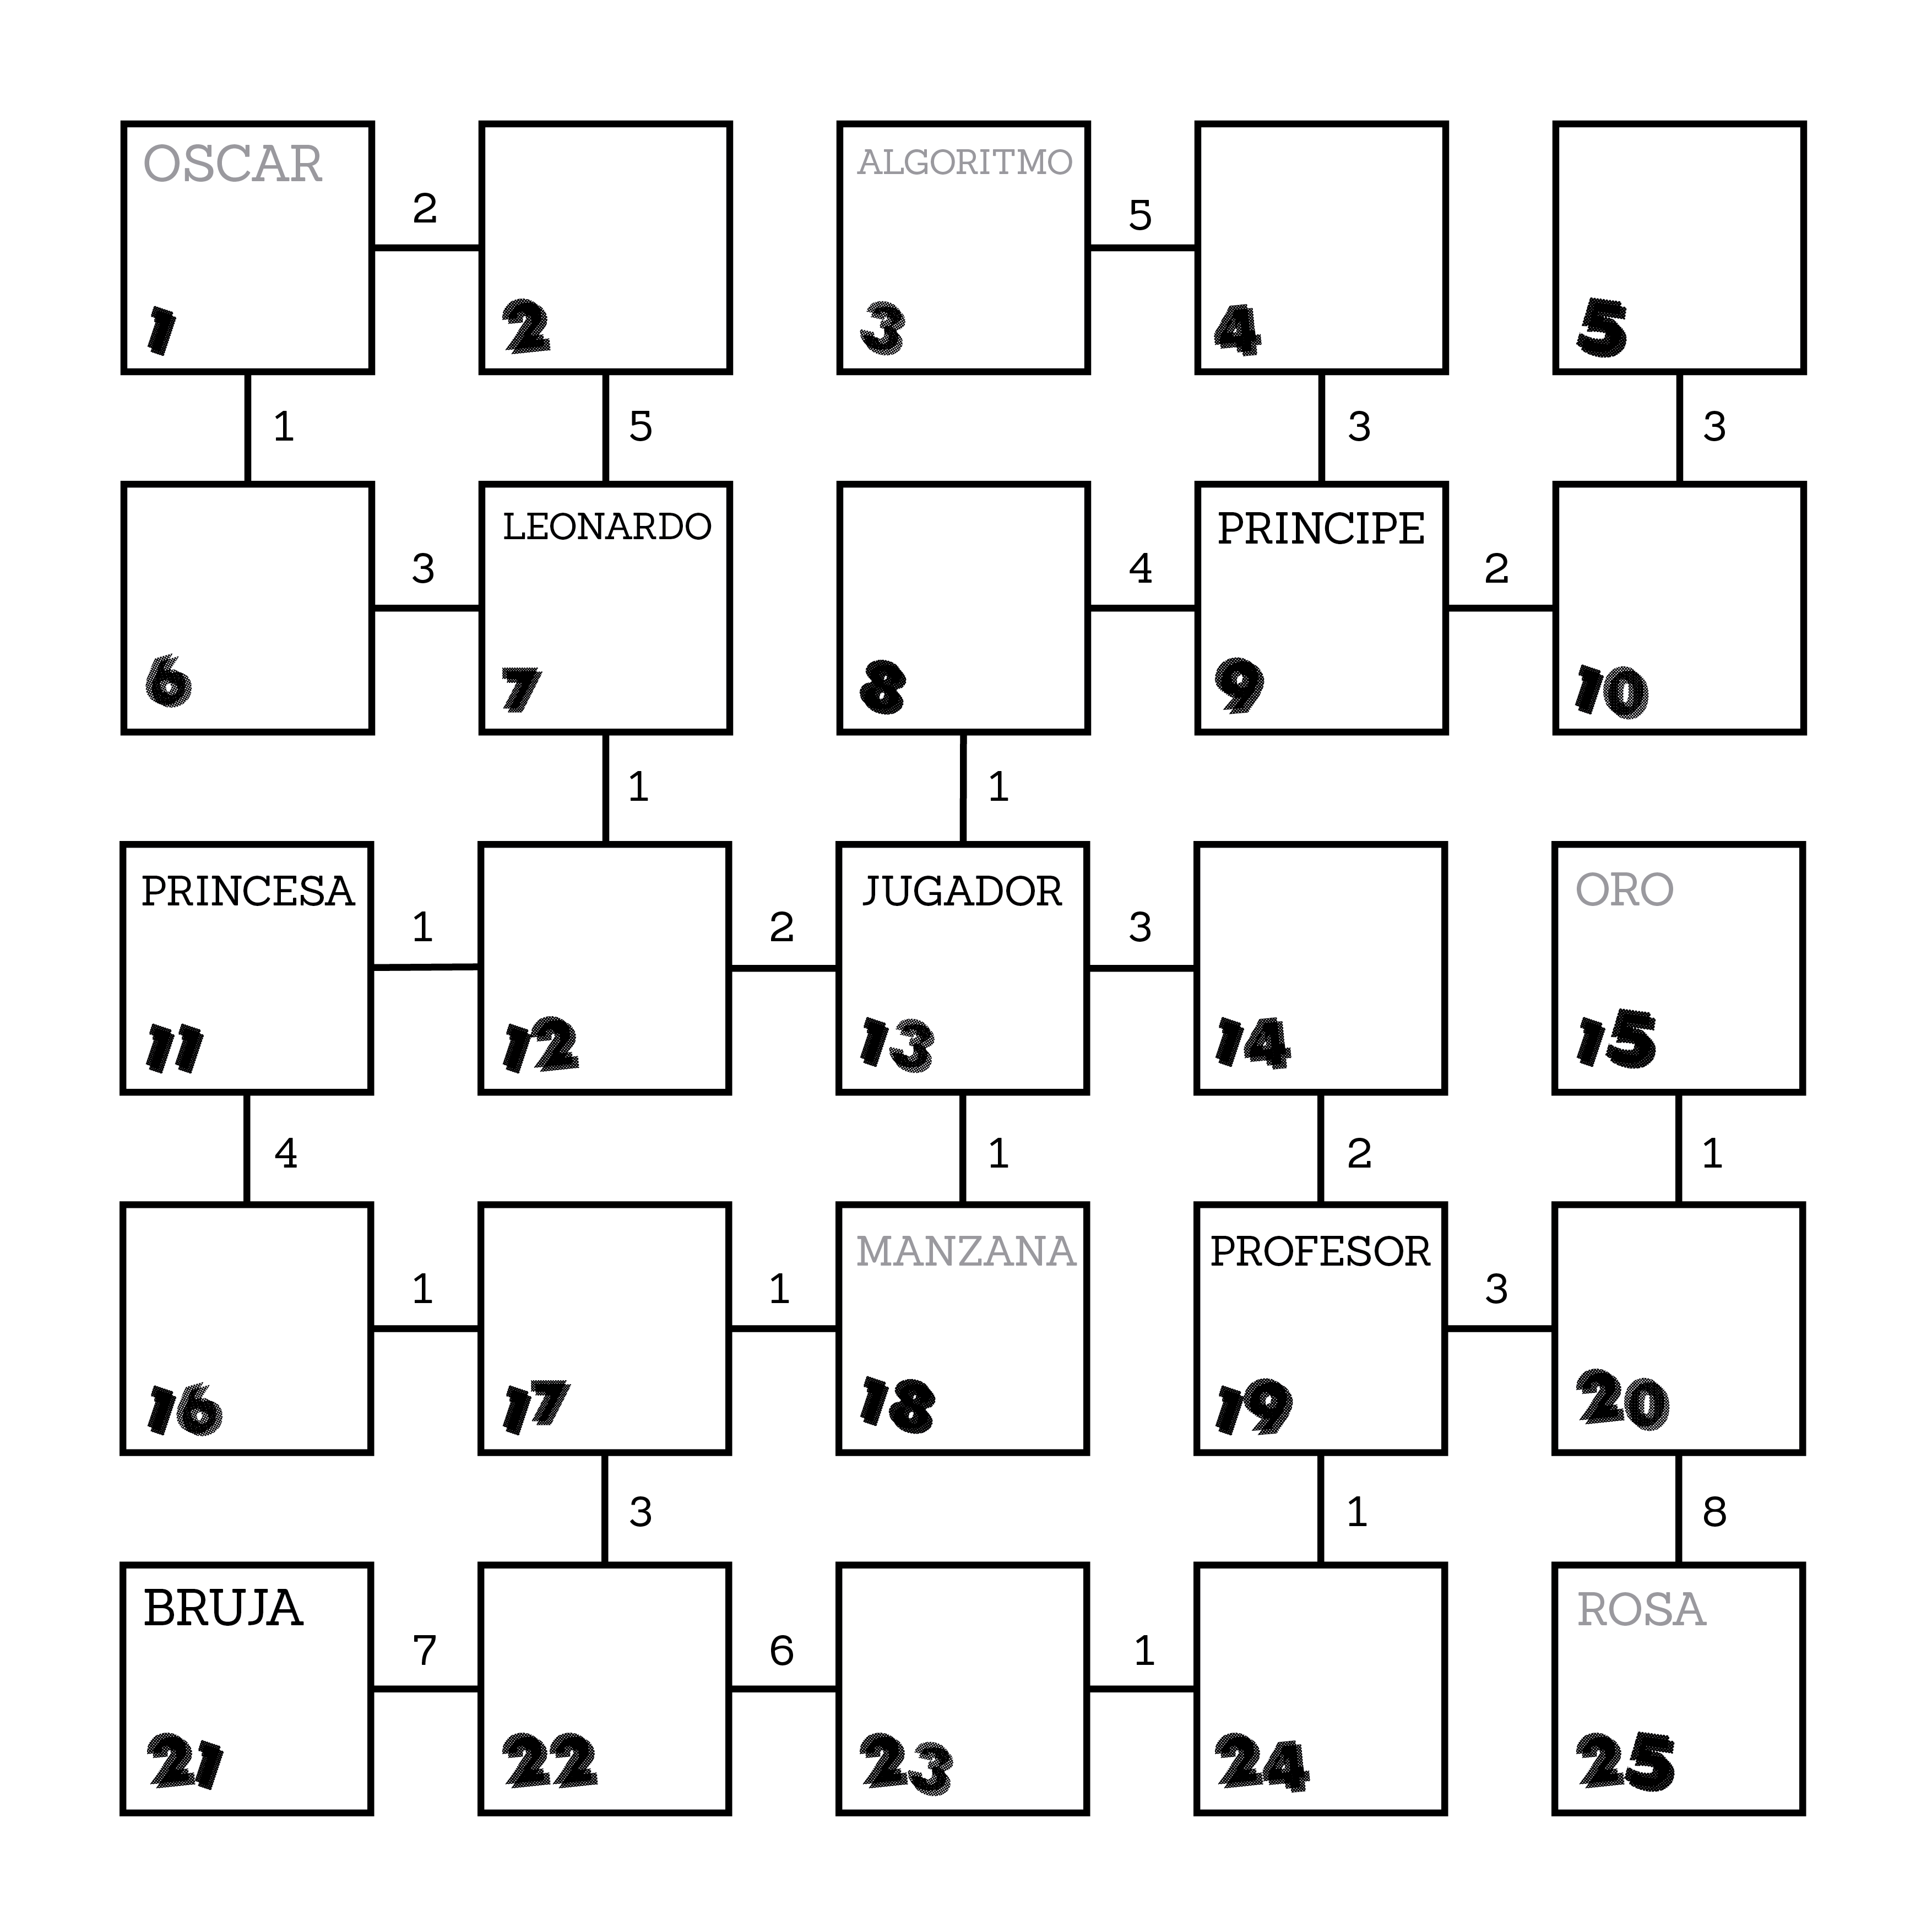
\includegraphics[scale=0.5]{img/e2.png}
\subsubsection{Apartado A}
En el ejercicio 2 se pide adecuar el dominio ya definido a la nueva característica de que los caminos tienen una 
longitud definida.

Para ello, se ha introducido una nueva función, \texttt{(distance)}, definida en el problema.
En la regla \texttt{GO}, al desplazarse se le suma al coste total del plan el valor definido de \texttt{(distance z1 z2)}.

\subsubsection{Apartado B}
En los problemas definidos para el dominio del ejercicio 2, ahora se indicará la distancia entre dos zonas, asignando el valor de
\texttt{(distance ?z1 ?z2)} junto con la declaración de los caminos. Por ejemplo, si hay un camino de distancia 3 entre z1 y z7, en 
el problema aparecería:

\texttt{(path z1 z7) (path z7 z1) (= (distance z1 z7) 3) (= (distance z7 z1) 3)}

\subsubsection{Apartado C}
El parser se ha ampliado para leer la distancia entre las zonas. Para ello, en lugar de guardar una 2-tupla con las zonas conectadas en el vector correspondiente, se guarda una 3-tupla, con las zonas y la distancia entre ellas. Posteriormente se interpreta y escribe en el 
fichero resultado.


\subsection{Ejercicio 3}
\subsubsection{Mapa de problema 1}
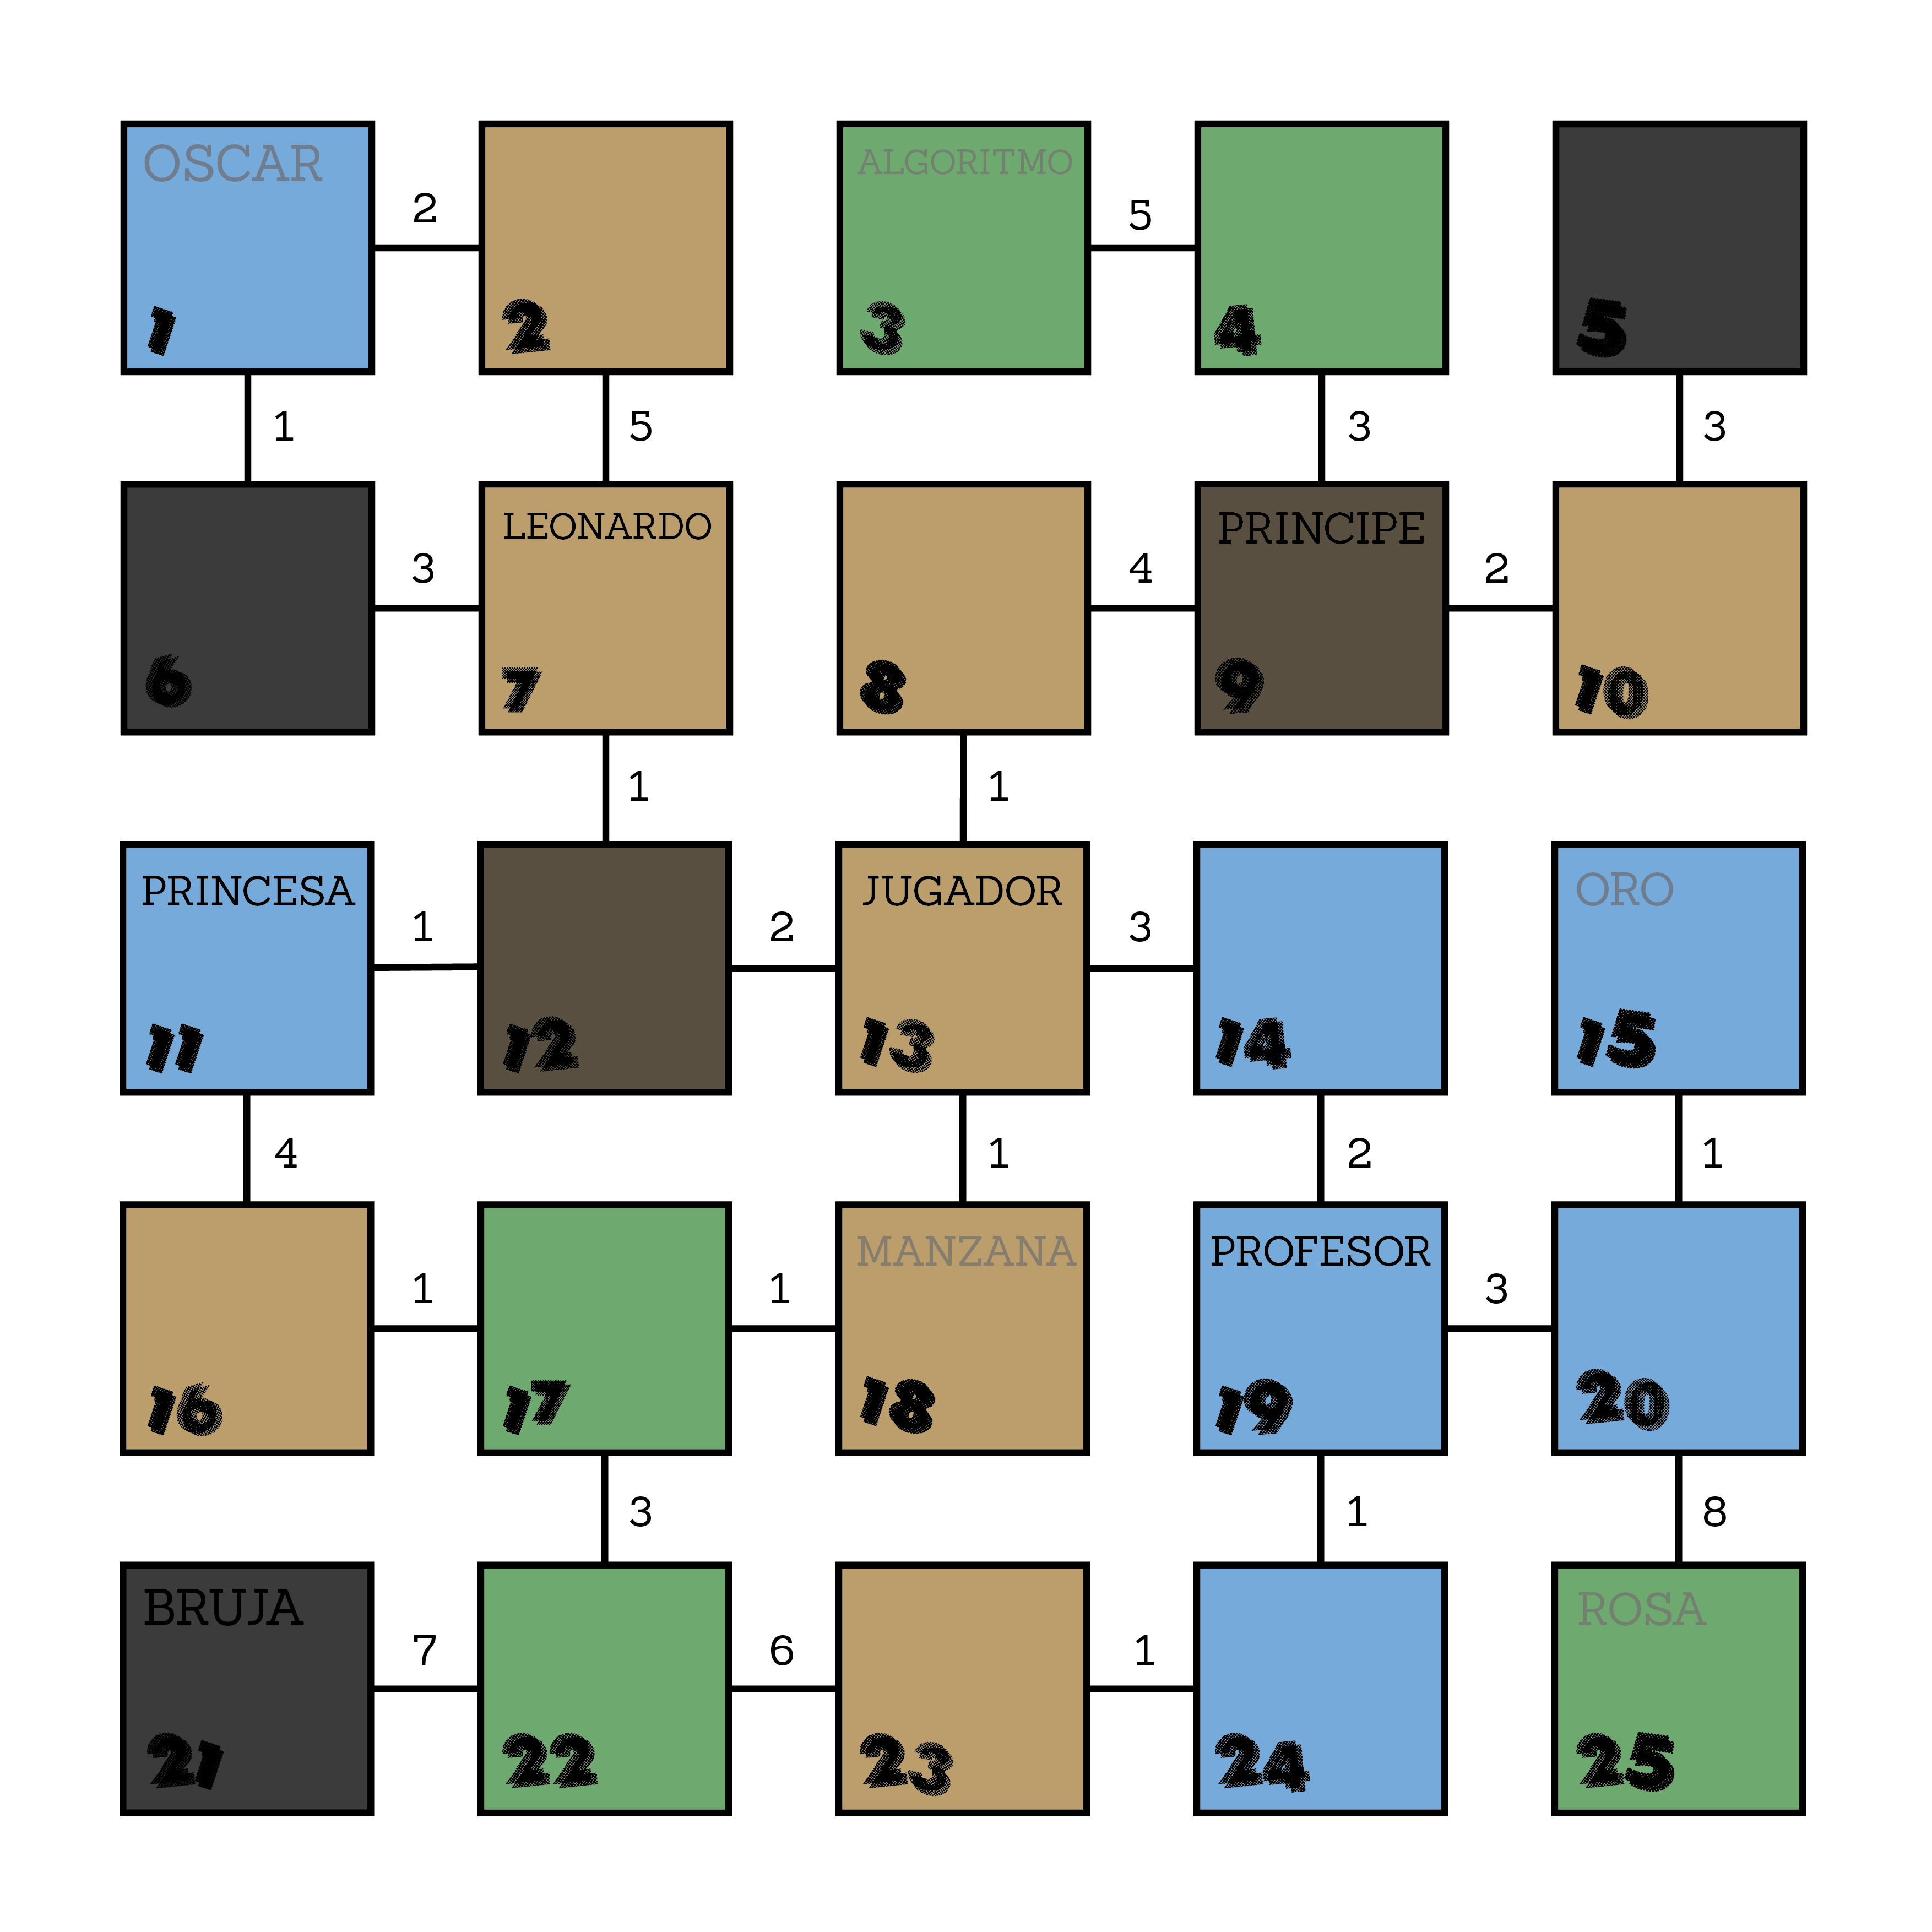
\includegraphics[scale=0.5]{img/e3.png}
\subsubsection{Apartados A y B}
En el ejercicio 3 se pide introducir terrenos a las diferentes zonas, necesitando objetos especiales para pasar por algunos de ellos. Además, ahora el jugador dispondrá de una mochila, en la que podrá guardar un objeto extra.


Se ha modificado la forma en la que se representan los objetos que tiene el jugador. Primero, si tiene la mano vacía, existirá en la 
base de hechos \texttt{(hand\_empty)}, y si lo está la mochila, \texttt{(bag,\_empty)}. 


Si tiene algo en la mano, existirá en la base de hechos \texttt{(on\_hand ?o - object)}, y lo mismo en la mochila con \texttt{(on\_bag ?o - object)}.


Si necesitamos pasar por terrenos por los que necesitamos ropa especial, comprobará si la tenemos en la mano o en la mochila en la acción \texttt{GO}.

\subsubsection{Apartado C}
En los problemas definidos para el dominio del ejercicio 3, se indicará el terreno de cada zona con el predicado \texttt{(room\_type ?z - room ?t - terrain)}.

\subsubsection{Apartado D}
El parser se ha ampliado para incorporar el tipo de terreno al problema. Si no se definen las zapatillas o el bikini, se situarán en una zona arbitraria.

\subsection{Ejercicio 4}
\subsubsection{Mapa de problema 1}
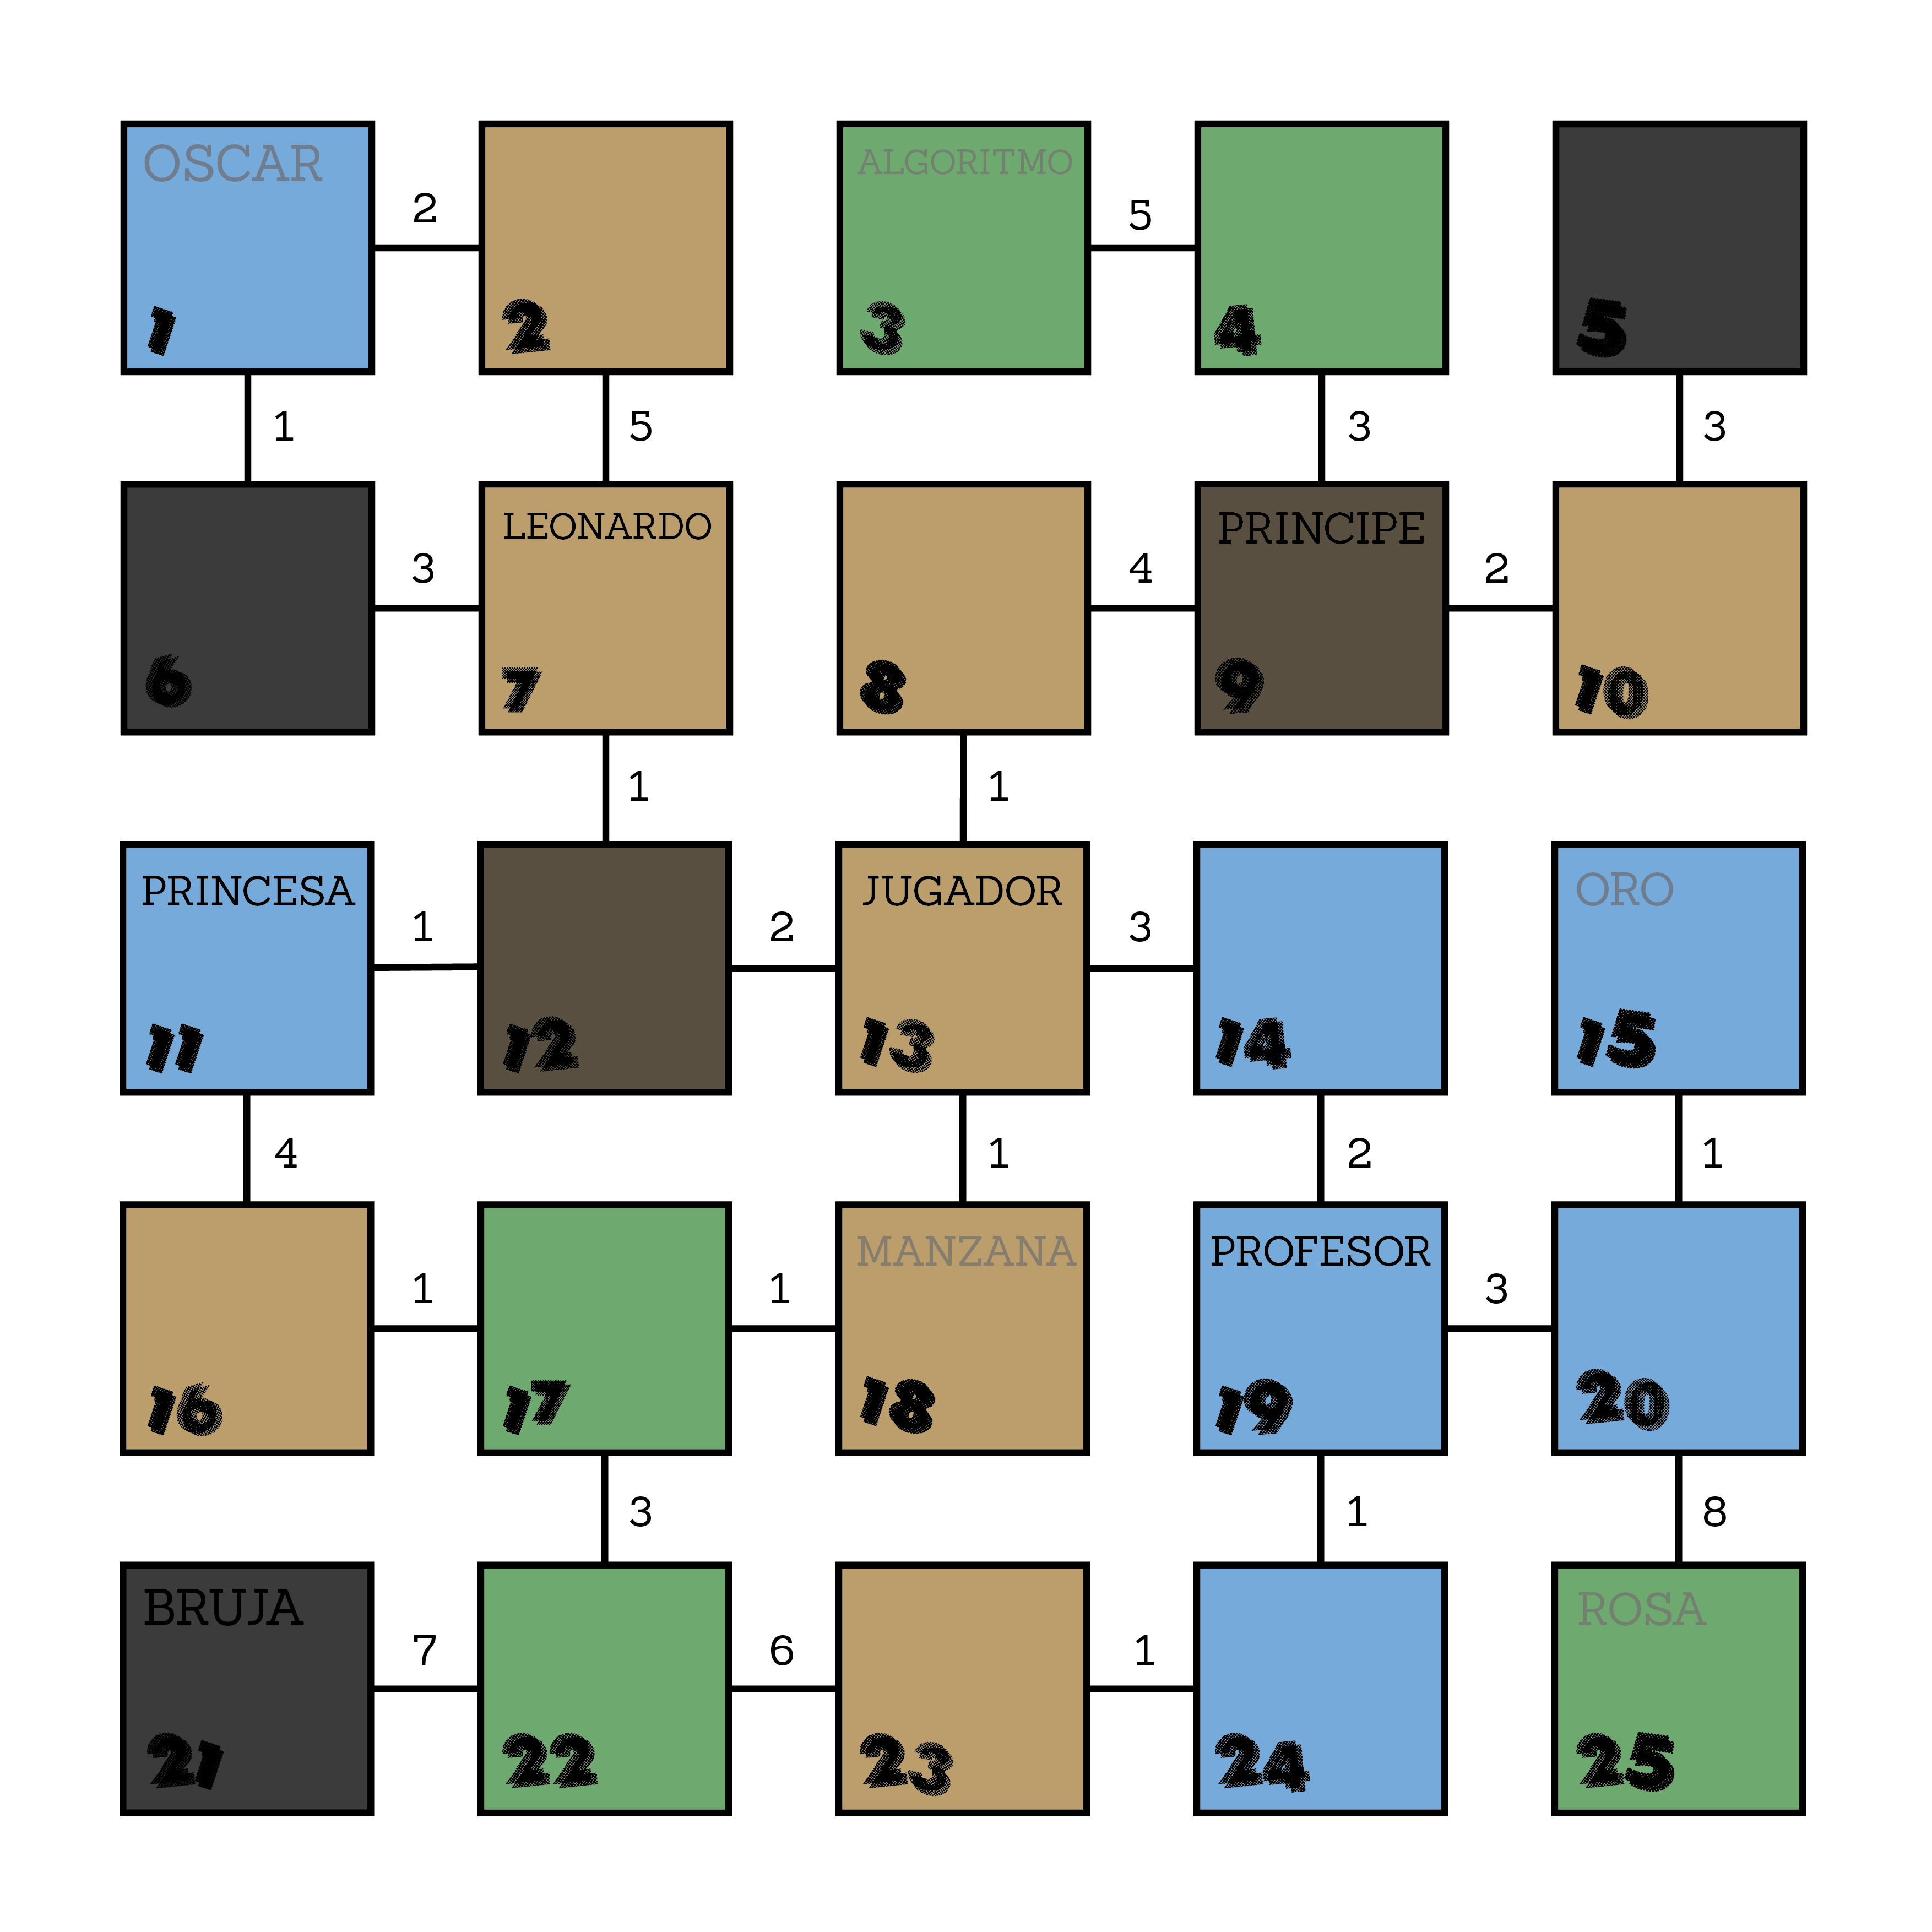
\includegraphics[scale=0.5]{img/e3.png}
\subsubsection{Apartado A}
En el ejercicio 4 se proporciona una tabla de puntuación, con la que se define cuántos puntos gana el jugador por entregar un
determinado objeto a un determinado personaje. El dominio se ha modificado añadiendo las funciones \texttt{(points\_given ?ch - npc ?o - object)} y \texttt{(points\_earned)}, que indican los puntos dados por un npc dado un objeto y los puntos totales acumulados, respectivamente.

\subsubsection{Apartado B}
La tabla se ha representado utilizando la función \texttt{(points\_given ?ch - npc ?o - object)}.

\subsubsection{Apartado C}
El parser se ha actualizado para leer los puntos a alcanzar e incluirlos como parte de la meta.

\subsection{Ejercicio 5}
\subsubsection{Mapa de problema 1}
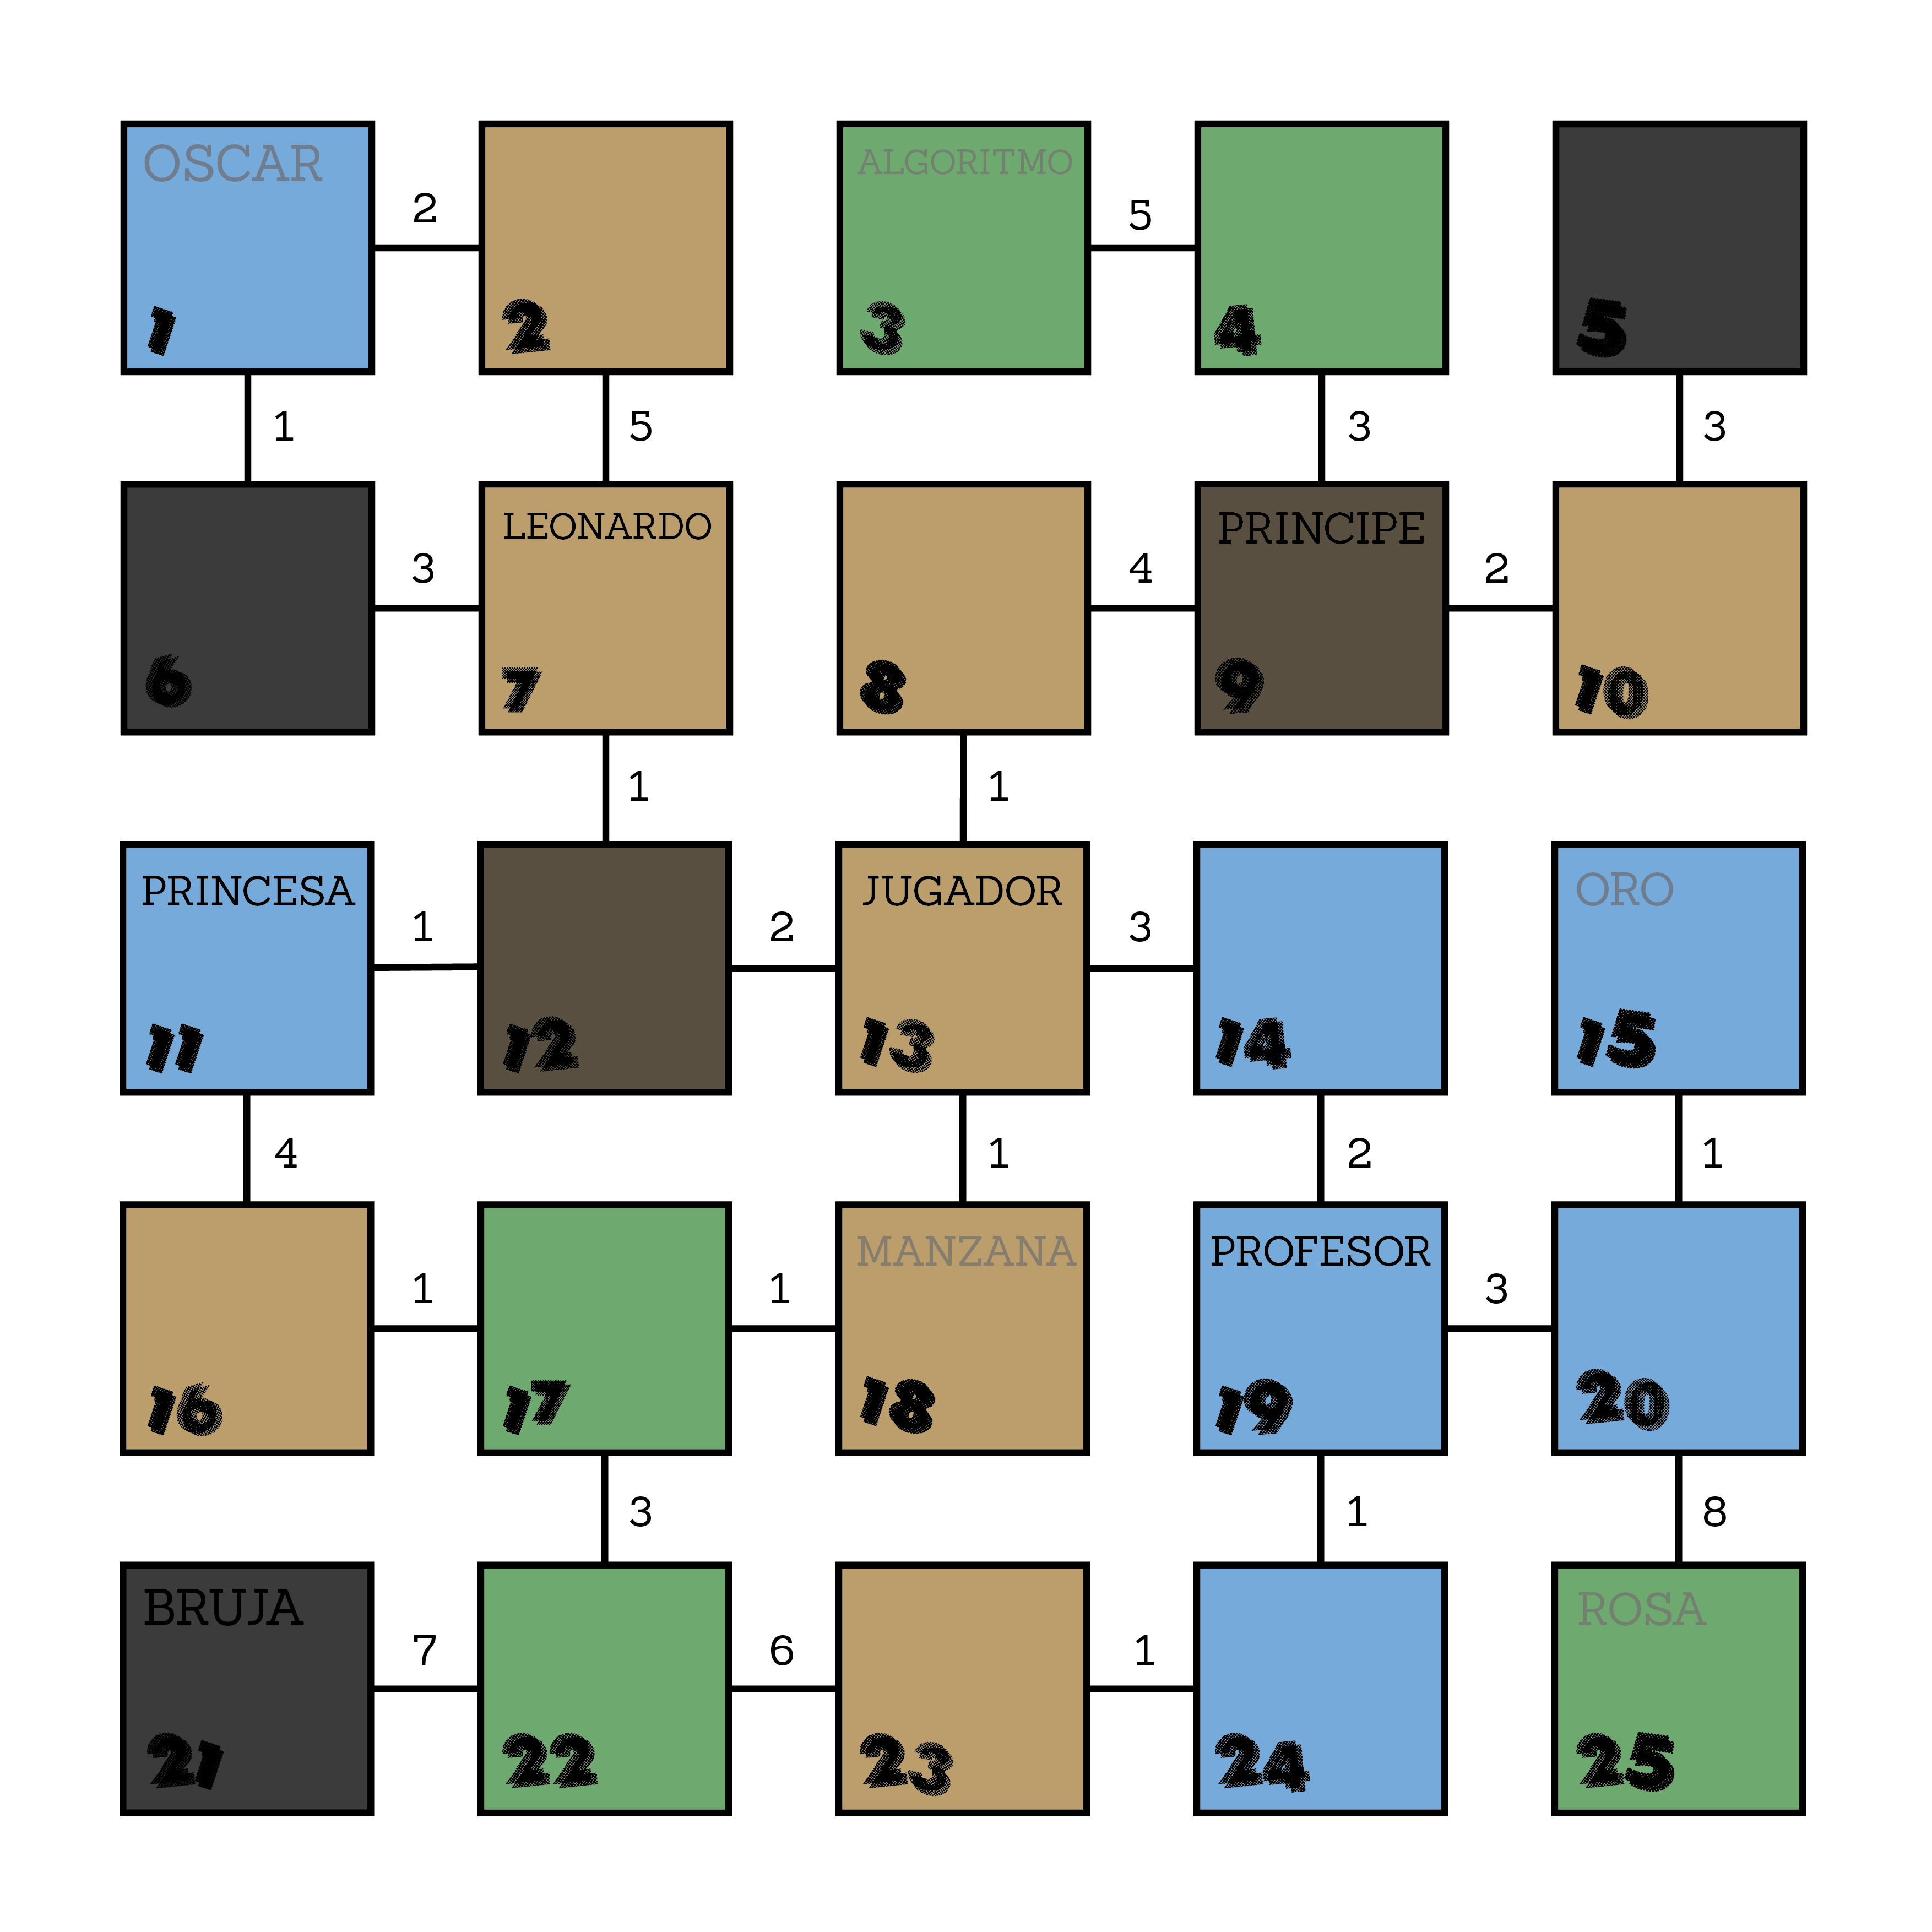
\includegraphics[scale=0.5]{img/e3.png}
\subsubsection{Apartado A}
Se ha ampliado el dominio anterior para representar el bolsillo de cada personaje añadiendo las funciones \texttt{(stock ?ch - npc)} y \texttt{(max\_stock ?ch - npc)}, que representan los objetos obtenidos y la capacidad máxima, respectivamente.

En la acción \texttt{GIVE}, se ha añadido que compruebe si el personaje tiene hueco para más objetos, y en caso de tenerlo, se le entregue y se incremente en uno el total de objetos. Si no, no puede entregarlo.

\subsubsection{Apartado B}
El problema se ha extendido añadiendo el stock máximo de los NPC, y comenzando todos con cero objetos. 

\subsubsection{Apartado C}
El parser se ha ampliado para representar el stock de cada personaje, añadiendo también que todos comienzan con cero objetos.

\subsection{Ejercicio 6}
\subsubsection{Mapa de problema 1}

\subsubsection{Apartado A}
En este ejercicio se ha introducido un nuevo jugador, y por tanto, todos los predicados que utilizábamos anteriormente para representar el estado del jugador ahora necesitan un parámetro. Se han modificado para que ambos jugadores puedan hacer uso de ellos. También se ha
añadido la función \texttt{(total\_points)}, para representar los puntos conseguidos en conjunto.

\subsubsection{Apartado B}
Se han indicado las condiciones iniciales del segundo jugador en el problema, y los puntos a conseguir.



\end{document}